\chapter{System Model}
\label{cha:system}
\vspace{0.4 cm}

In this chapter, the model of the proposed system is presented.
In the first section, an in-depth presentation of the designed system architecture is provided.
The different components of the system with their functionalities and interactions are described.
Tthe overall architecture was designed in order to build a Software as a Service (SaaS) solution capable of satisfying different use cases and being used directly by energy retailers.
Lastly, the modules focused on the three use cases of interest are treated more in detail in dedicated sections.
After this chapter, it will be clear what the main parts of the system are and how they cooperate to accomplish the various use cases of interest.


\section{System architecture}
\label{sec:architecture}
\vspace{0.2 cm}

The use case diagram for the proposed system is presented in figure~\ref{fig:usecase}.
Users can interact with the system via dedicated APIs.
To be authorized, a user must be authenticated and have an account with an active subscription.
Users can request the following asynchronous operations:
\begin{itemize}
  \item Load new data with a create or update logic specifying the type of data;
  \item Train new models based on available data for a specific use case specifying the time granularity (hourly or daily). The supported specific use cases for the models that will be used in the dedicated forecast requests are electricity demand forecasting, consumption baseline forecasting, and electricity production forecasting;
  \item Forecast future data for a specific use case using a specified model for a certain time granularity, for a certain starting date and time horizon.
\end{itemize}

In addition, a task scheduler periodically triggers the performance evaluation of the available models and if needed triggers the models re-training for having up-to-date models with respect to the user data so that they might perform better on future forecasts.

\begin{figure}[H]
\centering
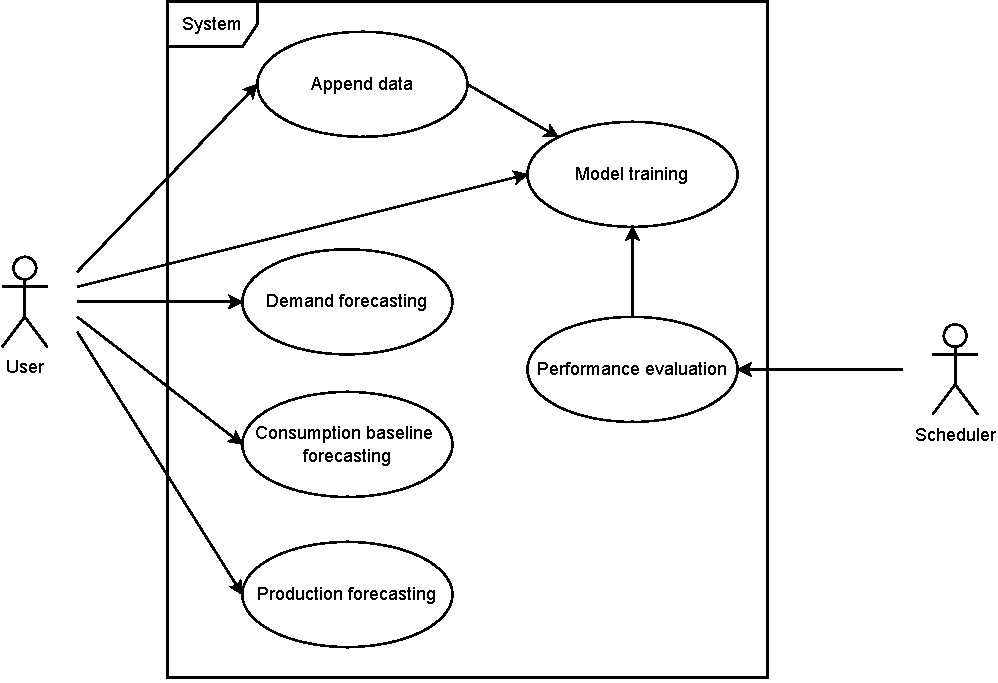
\includegraphics[width=0.6\textwidth]{images/architecture_use_case}
\caption{The use case diagram for the proposed system.}
\label{fig:usecase}
\end{figure}

For achieving the presented use cases the system architecture shown in figure~\ref{fig:components} was designed.
It is composed of the following components:
\begin{itemize}
  \item Authentication layer: manages the authentication process and verifies user permissions;
  \item API layer: manages the user interactions with the system;
  \item Task manager: coordinates the execution of the tasks;
  \item Data loading task: parses and stores the users' loaded data;
  \item ML models interface: handles the interactions with the ML models storage where the trained ML models are stored;
  \item Model training task: trains new models based on available data;
  \item Forecasting task: forecasts future data using a specified model;
  \item Task scheduler: manages the periodic scheduled tasks;
  \item Performance evaluation task: evaluates the performance of the available models and if needed triggers the models re-training.
\end{itemize}

The system interacts with the following external components:
\begin{itemize}
  \item Users data storage: used to store and retrieve user data, including account data;
  \item Data storage: used to store and retrieve the users' loaded data;
  \item Weather data storage: used to retrieve the weather data;
  \item ML models storage: used to store and retrieve the trained models;
  \item Forecasts storage: used to store and retrieve the computed forecasts.
\end{itemize}

\begin{figure}[H]
\centering
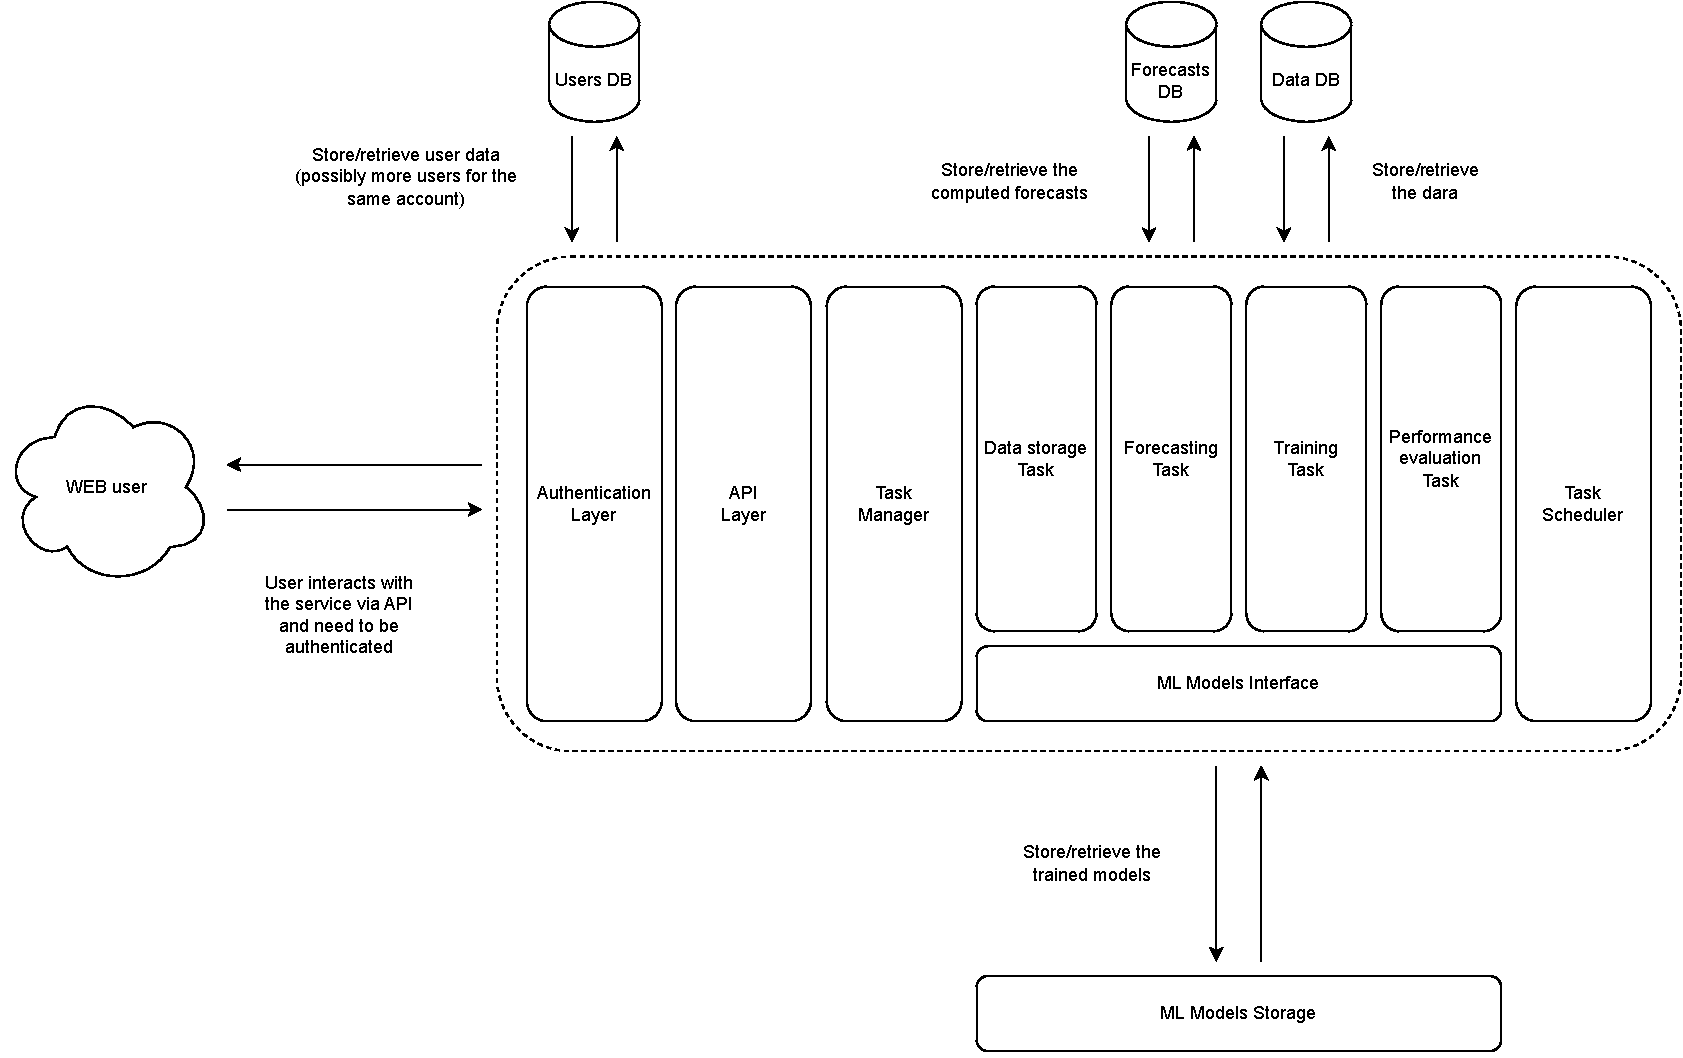
\includegraphics[width=0.9\textwidth]{images/architecture_components}
\caption{The architecture designed for the proposed system.}
\label{fig:components}
\end{figure}

Figure~\ref{fig:interactions} shows the interactions among the components of the designed architecture for achieving the presented use cases.
In the following subsections, the logic for each use case is explained with the relative components' interactions.

\begin{figure}[H]
\centering
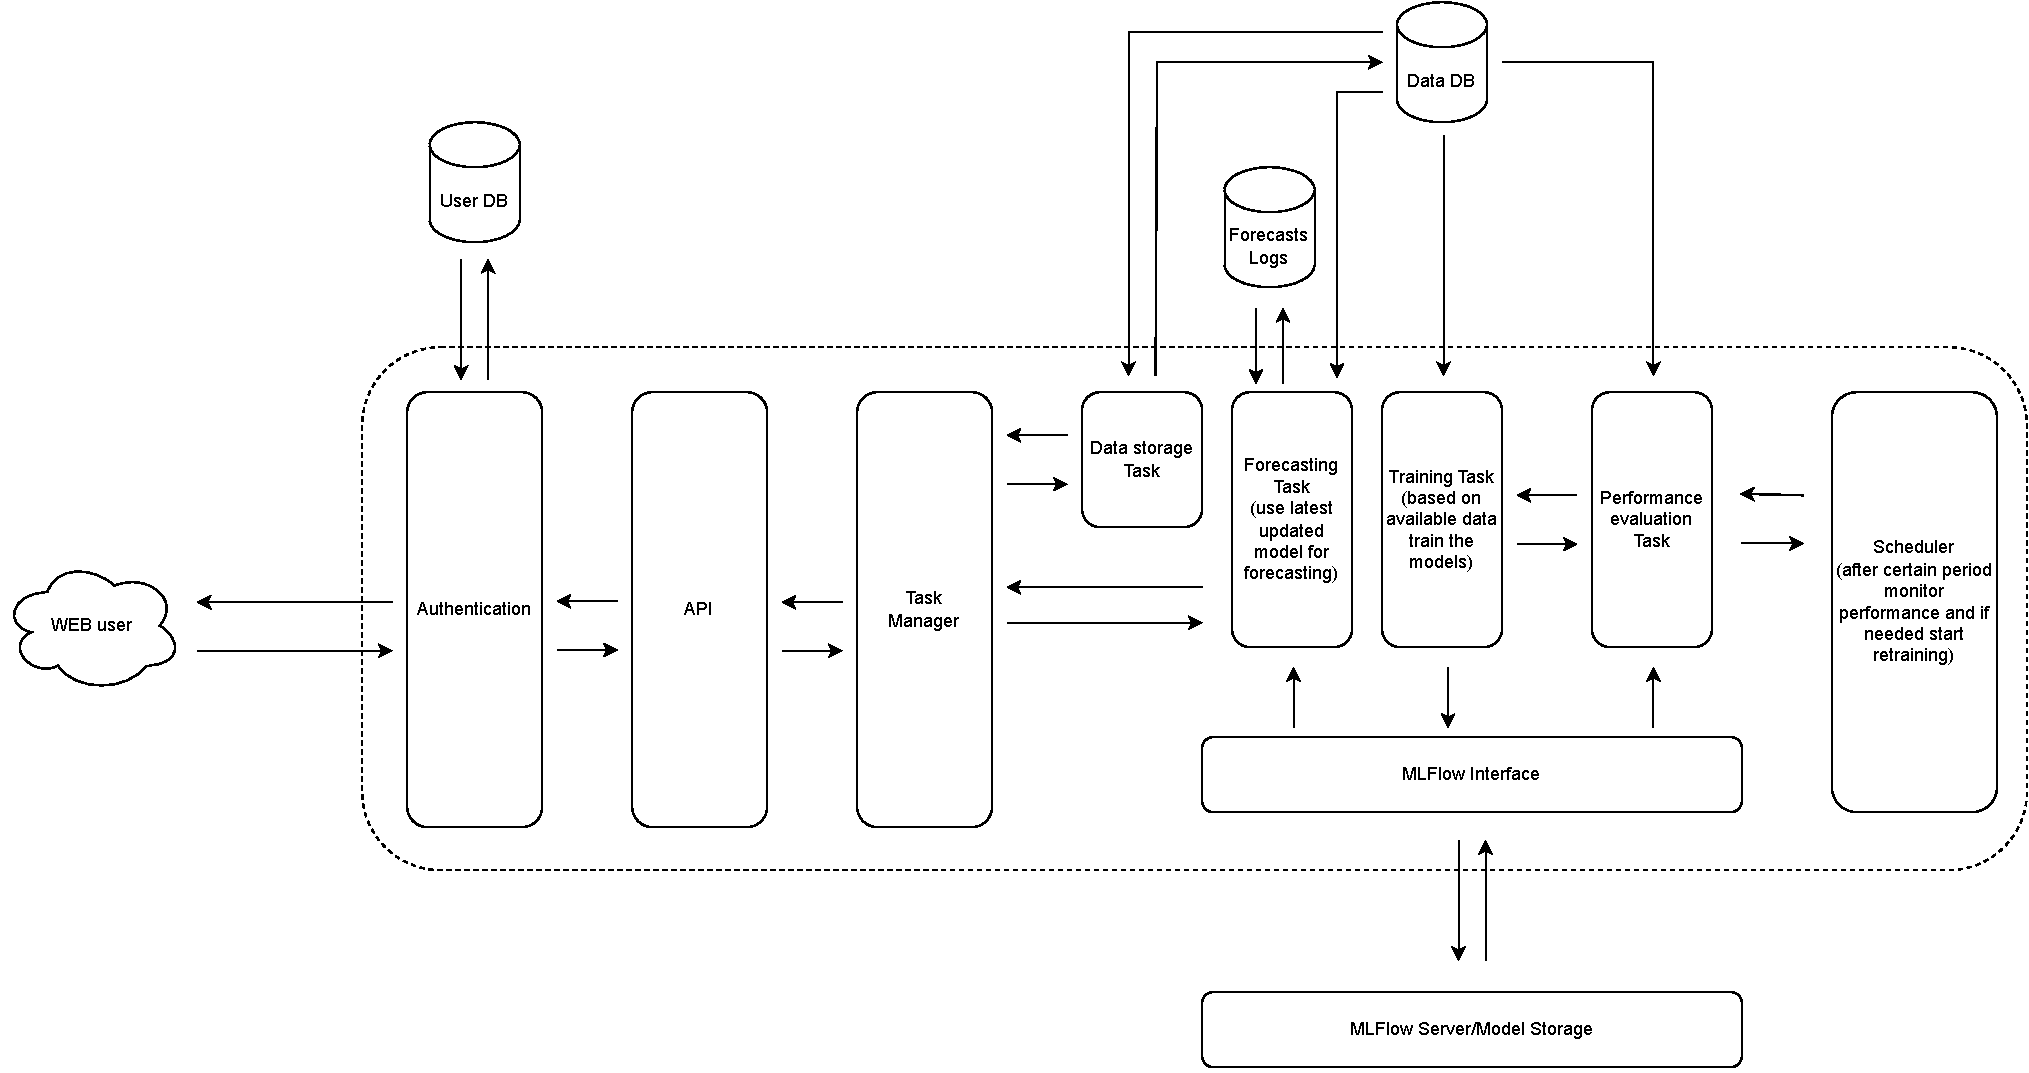
\includegraphics[width=1\textwidth]{images/architecture_interactions}
\caption{The interactions among the components in the designed architecture.}
\label{fig:interactions}
\end{figure}


\vspace{0.1 cm}
\subsection{Data loading}
\label{sec:loading}
\vspace{0.1 cm}

The diagram representing the components' interactions for achieving the data loading use case is presented in figure~\ref{fig:loadinginteractions}.

\begin{figure}[H]
\centering
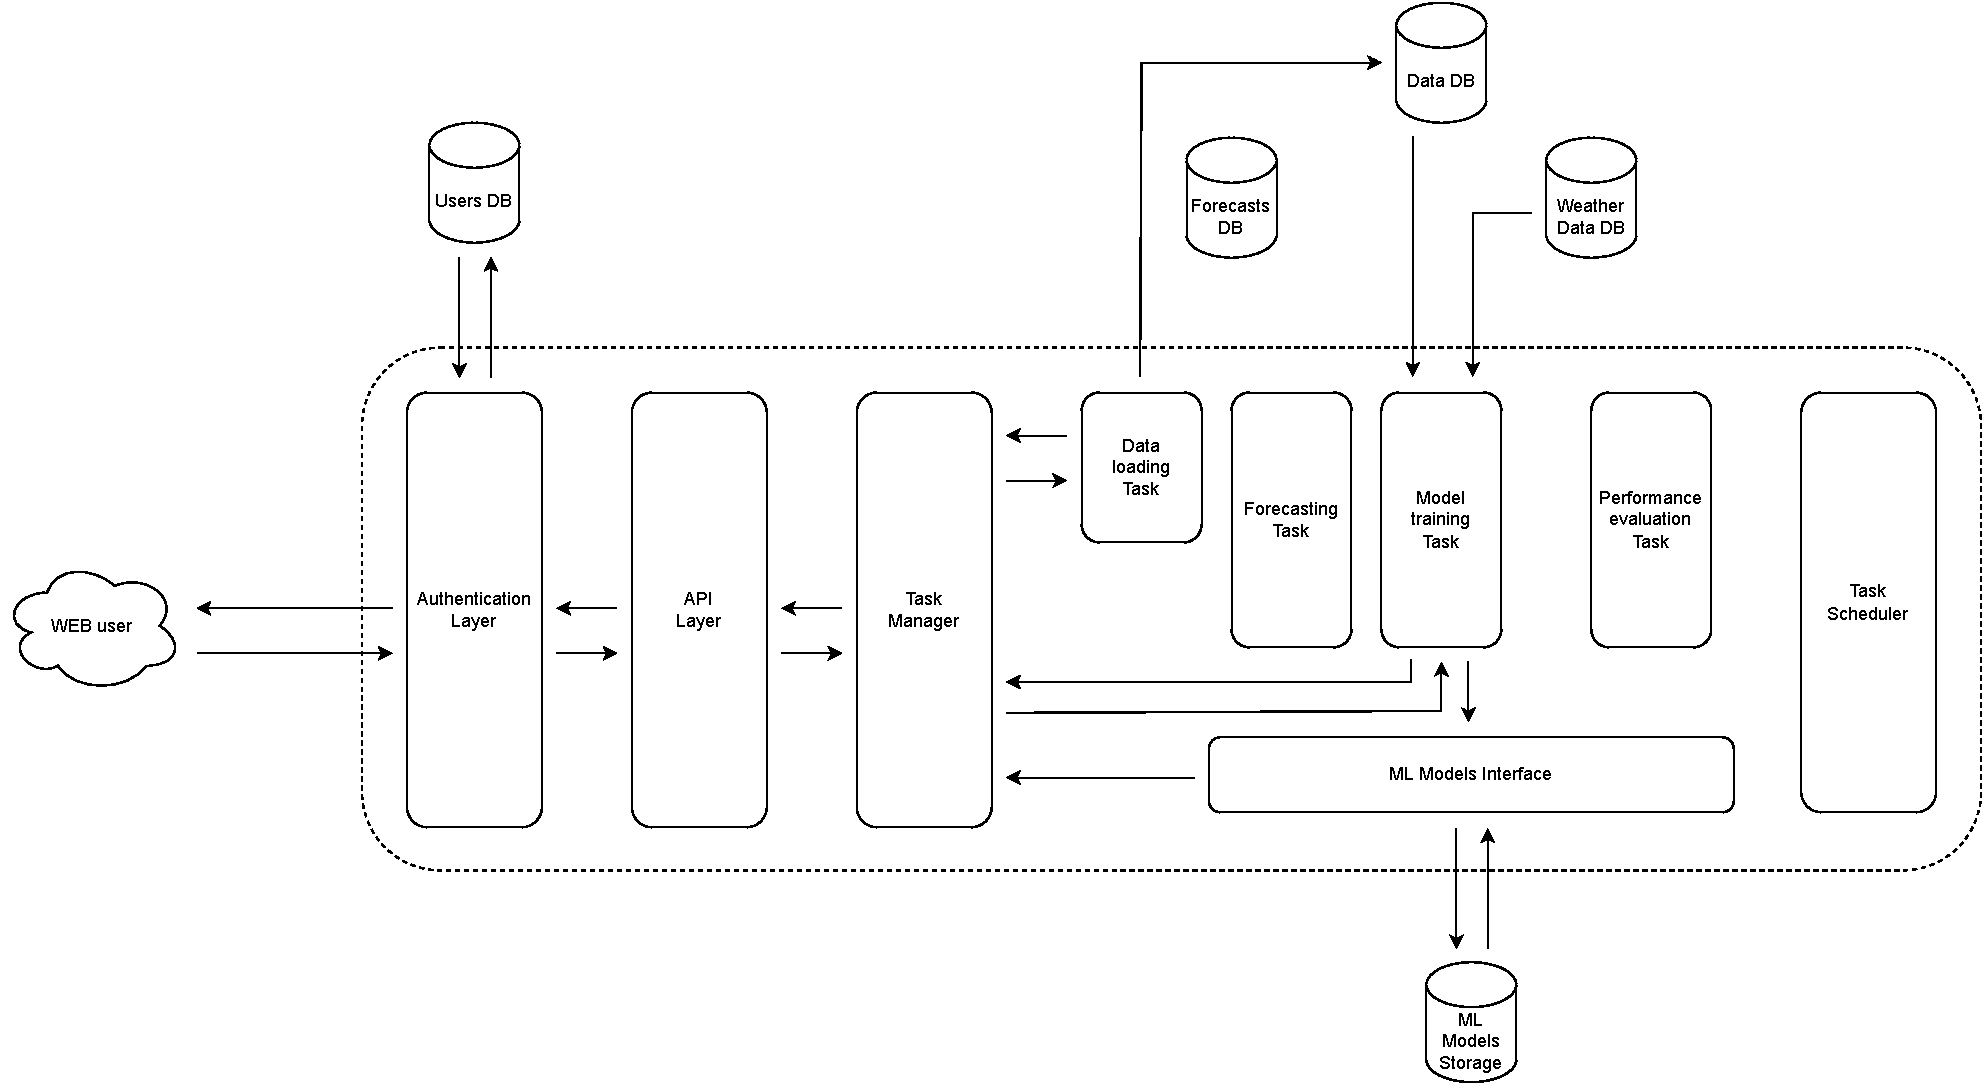
\includegraphics[width=1\textwidth]{images/architecture_data_loading_interactions}
\caption{The interactions among the components for achieving the data loading use case.}
\label{fig:loadinginteractions}
\end{figure}

The user sends the data to the system, for example uploading CSV files.
First, the authentication layer verifies the authentication of the user and checks whether it has a subscription to load the data.
The endpoint dedicated to data loading takes charge of the user request and provides the task manager with the details for creating a data loading task.
The identifier of the task is then returned to the user, who can request the status of the data loading request and check the result of the operation when completed.

The data loading task starts when the task manager schedules it.
As shown by the diagram in figure~\ref{fig:loadingflow}, the logic inside this task can be formulated in 2 steps: parse the data and store the data.
The data parser block transforms the user data in a system-compatible format and passes it to the data storage block which stores the data inside the data storage.
If there is no model for the specific use case for which data is loaded, the task manager will also create a model training task to train all the available models on this data.
This allows the system to be ready for the forecast requests on the loaded data.
The model training task is described more in detail in subsection~\ref{sec:training}.

\begin{figure}[H]
\centering
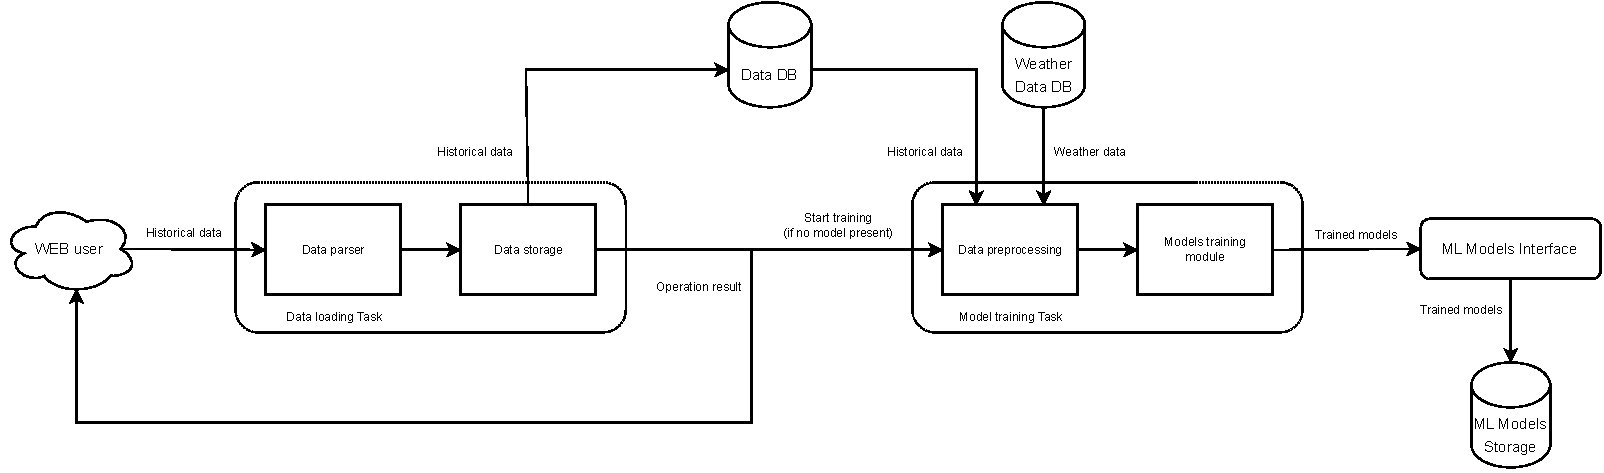
\includegraphics[width=1\textwidth]{images/architecture_data_loading_flow}
\caption{Diagram representing the data loading flow.}
\label{fig:loadingflow}
\end{figure}

The sequence diagram representing the complete data loading procedure is presented in figure~\ref{fig:loadingsequence}.

\begin{figure}[H]
\centering
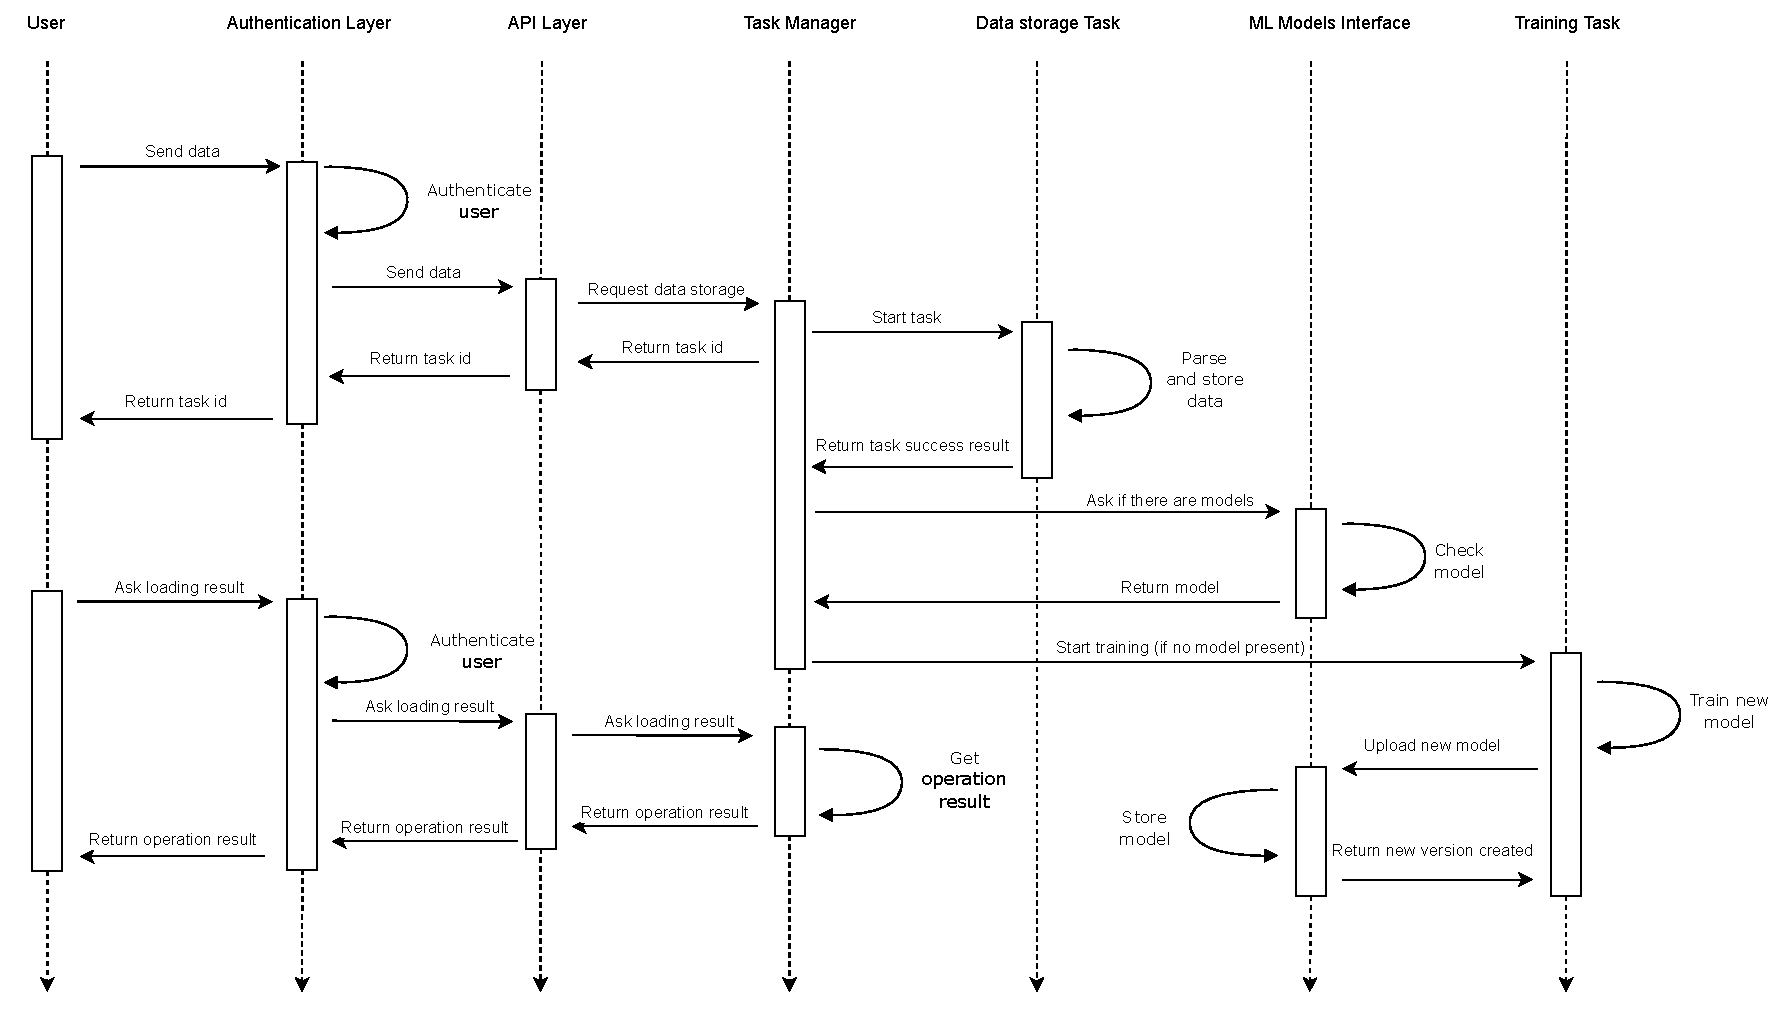
\includegraphics[width=1\textwidth]{images/architecture_data_loading_sequence}
\caption{Sequence diagram of the data loading procedure.}
\label{fig:loadingsequence}
\end{figure}


\vspace{0.1 cm}
\subsection{Model training}
\label{sec:training}
\vspace{0.1 cm}

The diagram representing the components' interactions for achieving the model training use case is presented in figure~\ref{fig:traininginteractions}.

The user sends the specification of the model to train to the system.
First, the authentication layer verifies the authentication of the user and checks whether it has a subscription to request the training of a model.
The endpoint dedicated to model training takes charge of the user request and provides the task manager with the details for creating a model training task.
The identifier of the task is then returned to the user, who can request the status of the model training request and get the trained model when completed.

\begin{figure}[H]
\centering
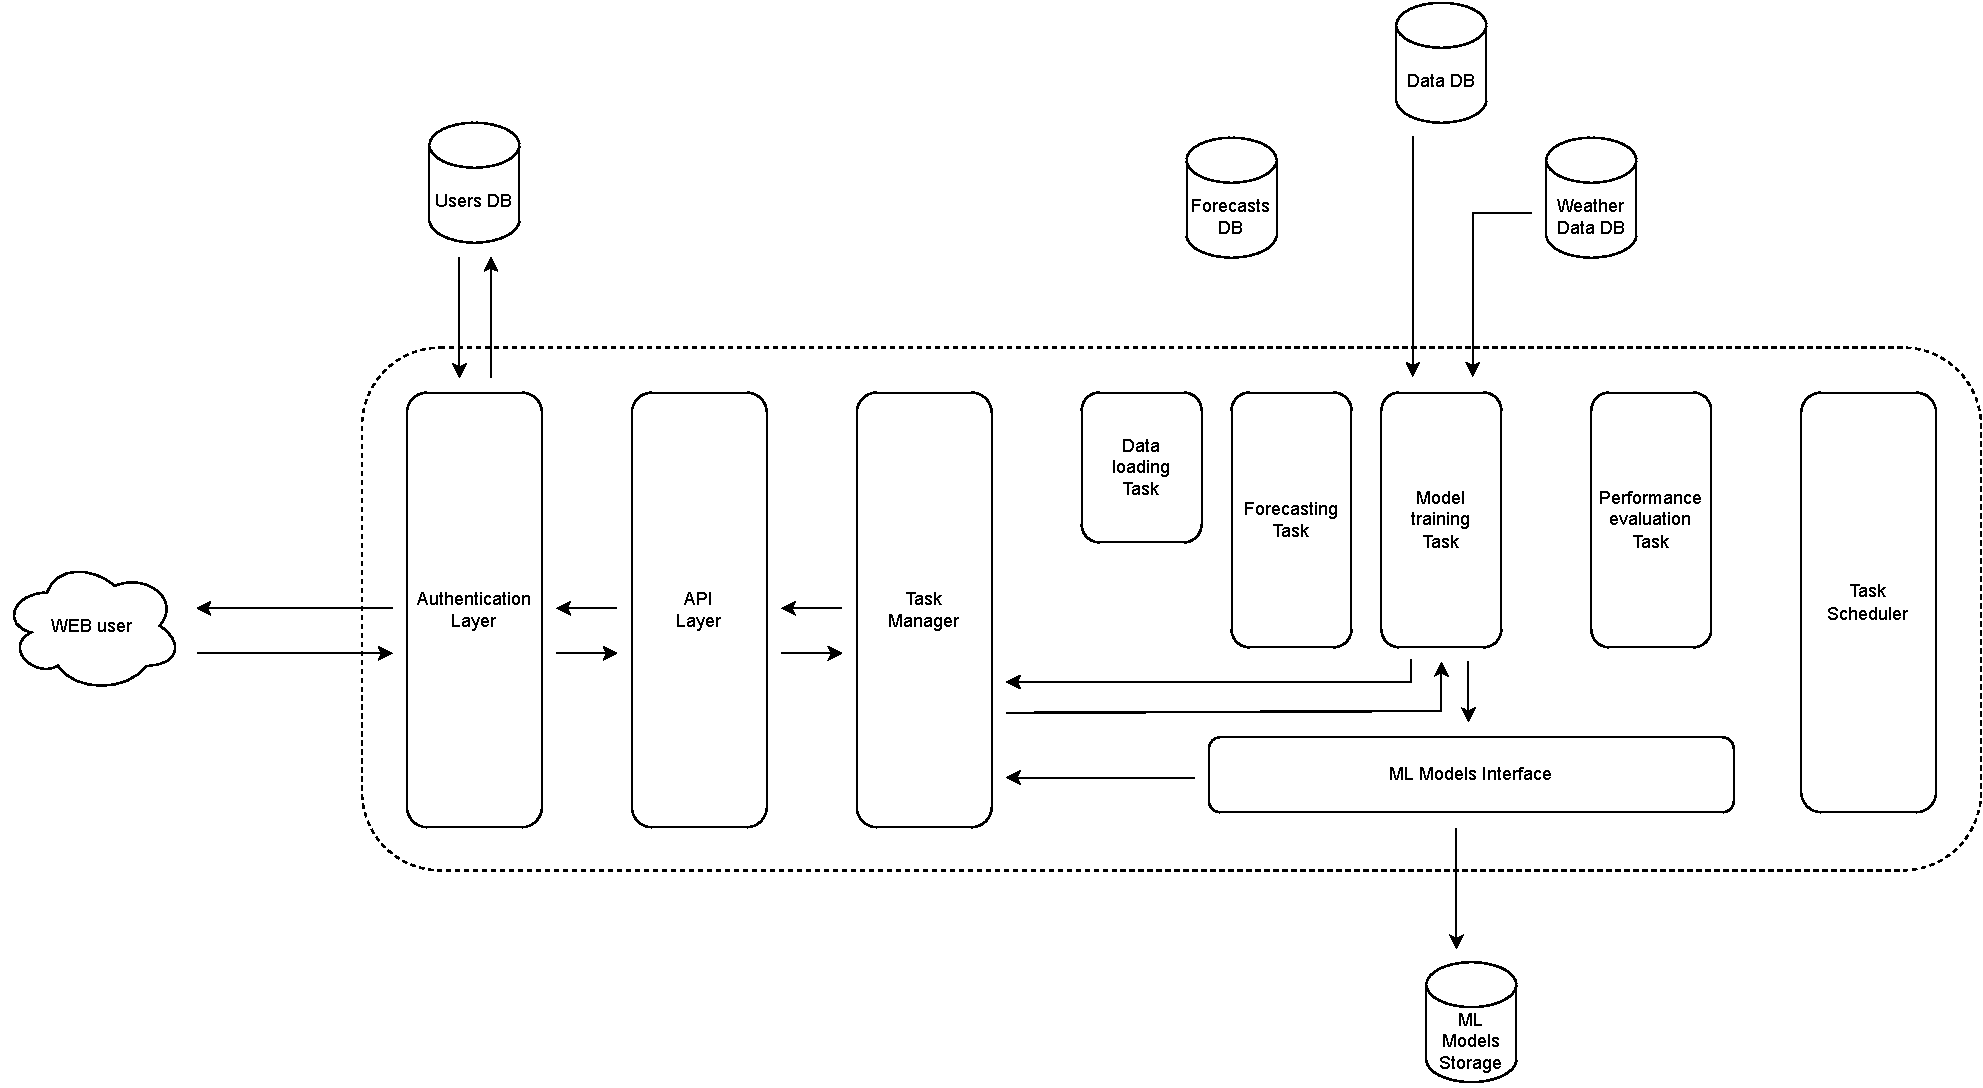
\includegraphics[width=1\textwidth]{images/architecture_training_interactions}
\caption{The interactions among the components for achieving the model training use case.}
\label{fig:traininginteractions}
\end{figure}

The model training task starts when the task manager schedules it.
As shown by the diagram in figure~\ref{fig:trainingflow}, the logic inside this task can be formulated in 2 steps: preprocess the available data and train the model.
The data preprocessing block collects the available data for the specific use case for which the model will be trained, aggregates it correctly, cleans it, and enriches it with weather data.
The models training module takes the preprocessed data and trains the model with the provided specifications.
It was thought of as an extendable framework on which it is possible to support different models and possibly integrate new ones over time.
The resulting model is then passed to the ML models interface which stores it inside the ML models storage.

\begin{figure}[H]
\centering
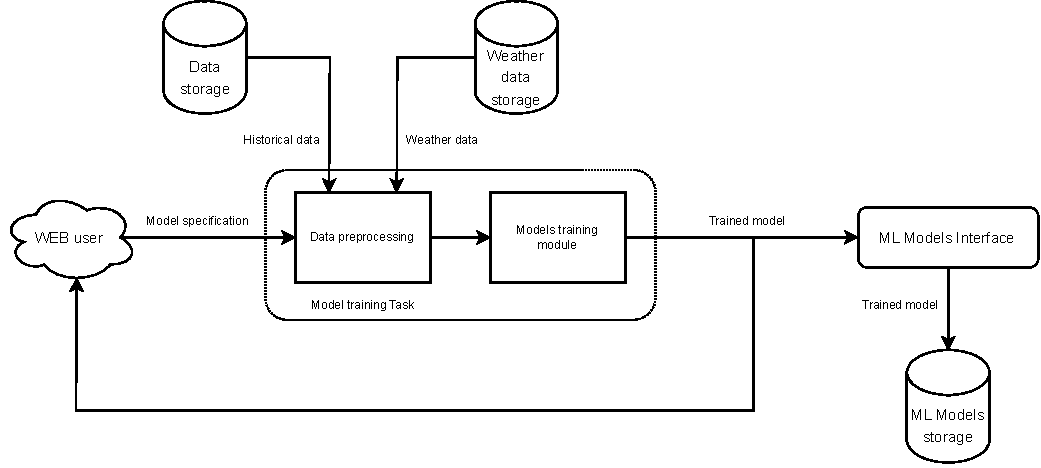
\includegraphics[width=0.7\textwidth]{images/architecture_training_flow}
\caption{Diagram representing the model training flow.}
\label{fig:trainingflow}
\end{figure}

The sequence diagram representing the complete model training procedure is presented in figure~\ref{fig:trainingsequence}.

\begin{figure}[H]
\centering
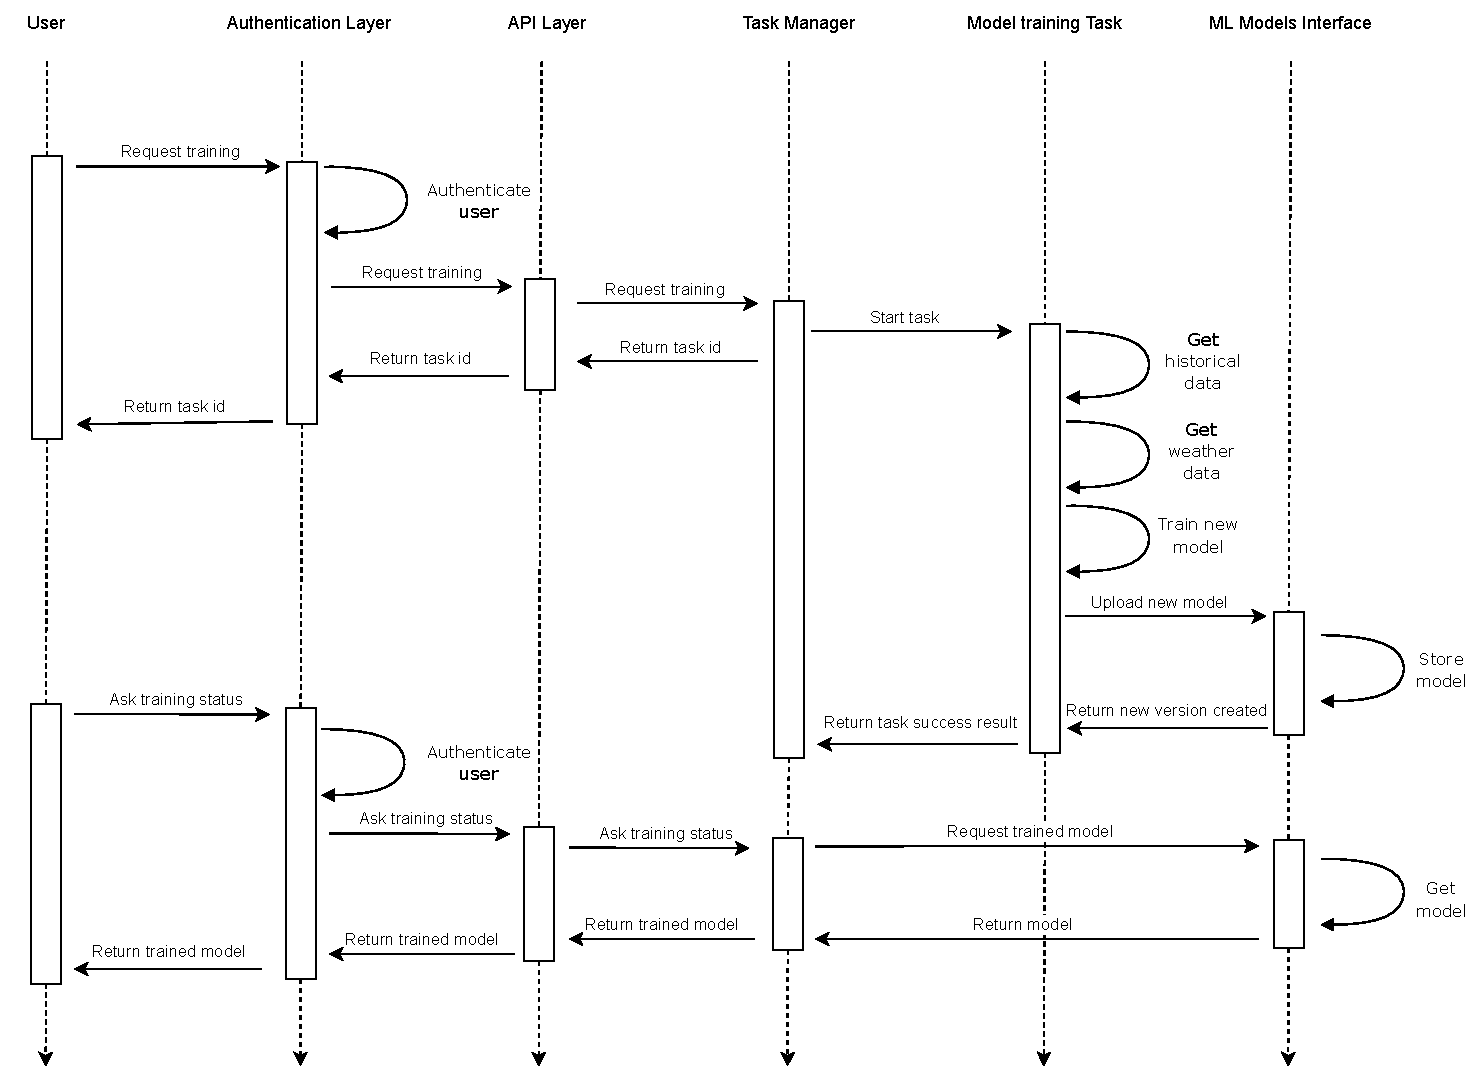
\includegraphics[width=0.8\textwidth]{images/architecture_training_sequence}
\caption{Sequence diagram representing the model training procedure.}
\label{fig:trainingsequence}
\end{figure}


\vspace{0.1 cm}
\subsection{Forecasting}
\label{sec:forecasting}
\vspace{0.1 cm}

The diagram representing the components' interactions for achieving the forecasting for a specific use case is presented in figure~\ref{fig:forecastinginteractions}.

\begin{figure}[H]
\centering
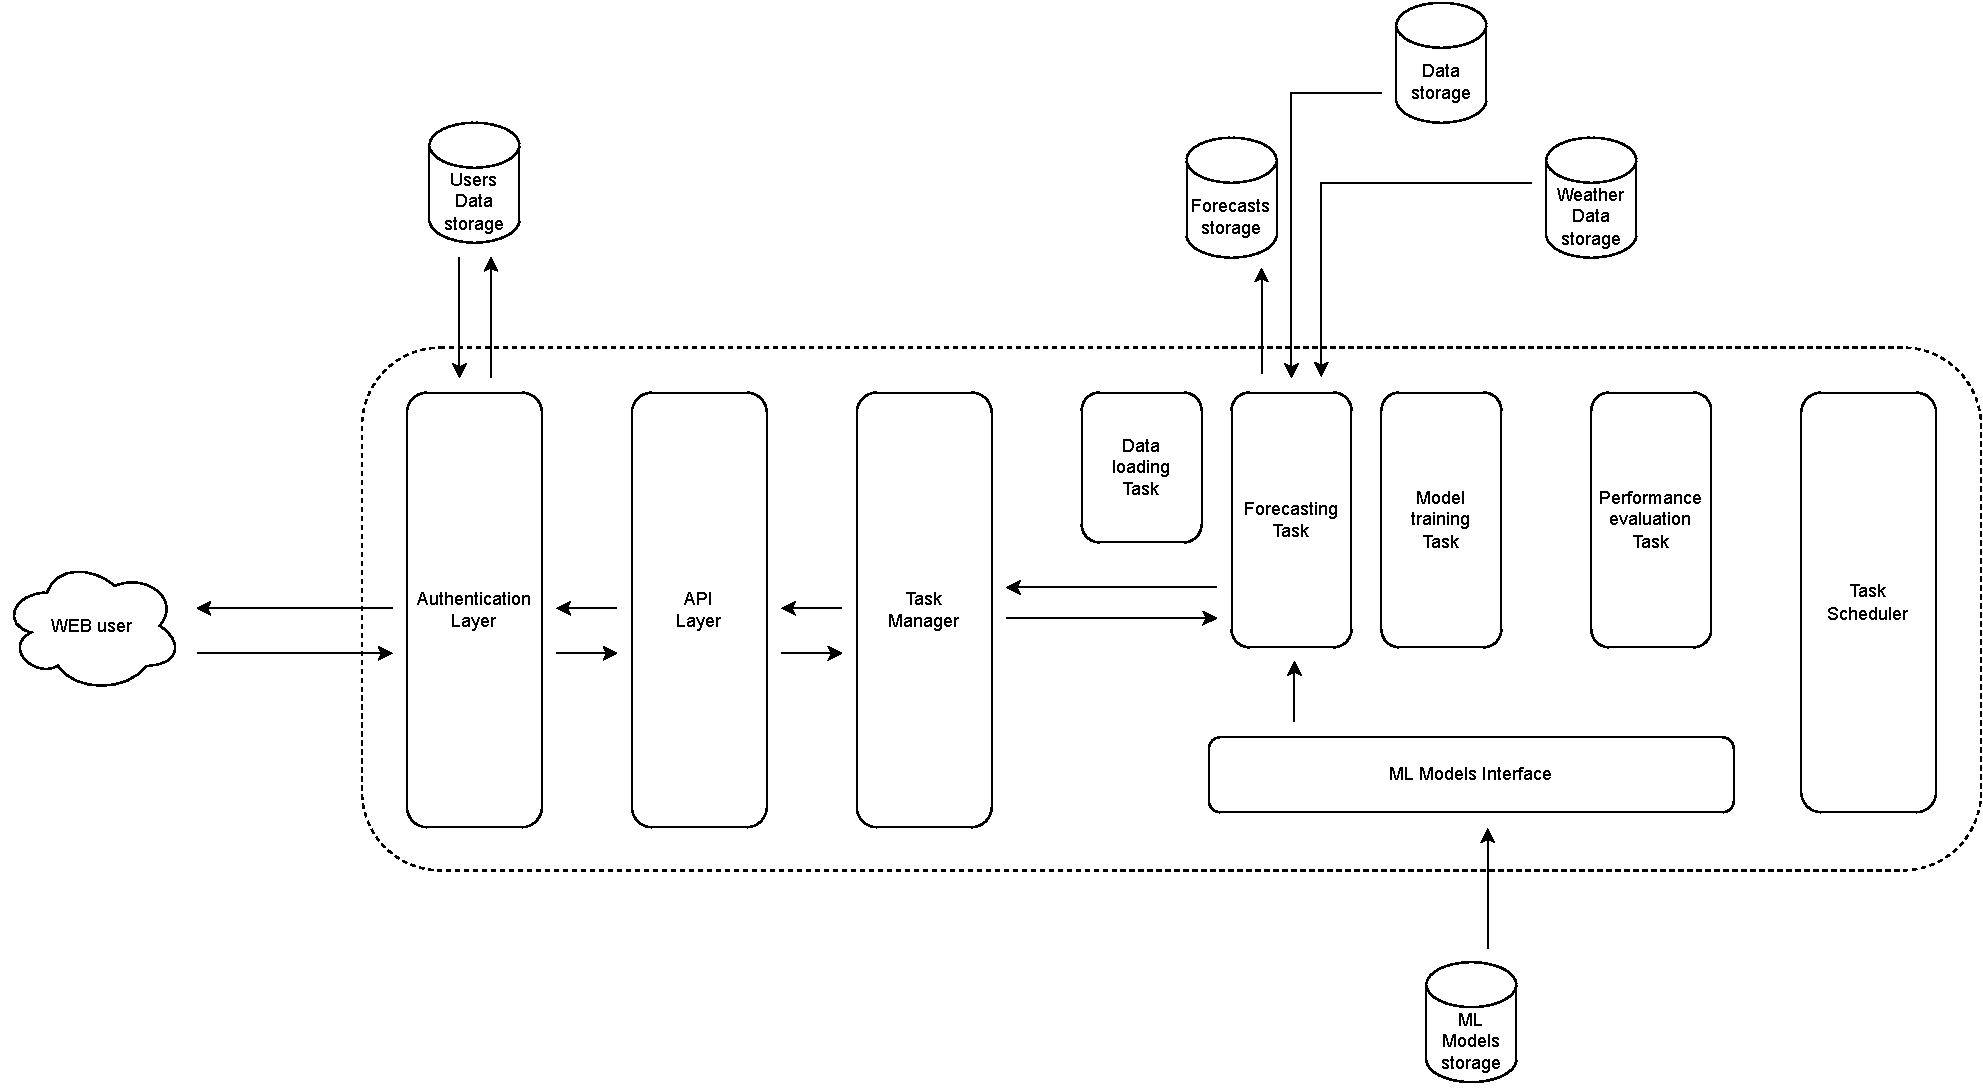
\includegraphics[width=1\textwidth]{images/architecture_forecasting_interactions}
\caption{The interactions among the components for achieving the forecasting for a specific use case.}
\label{fig:forecastinginteractions}
\end{figure}

The user sends the specification for computing forecasts for a specific use case to the system.
First, the authentication layer verifies the authentication of the user and checks whether it has a subscription to request the forecasts for a specific use case.
The endpoint dedicated to forecasting takes charge of the user request and provides the task manager with the details for creating a forecasting task.
The identifier of the task is then returned to the user, who can request the status of the forecasting request and get the computed forecasts when completed.

The forecasting task starts when the task manager schedules it.
As shown by the diagram in figure~\ref{fig:forecastflow}, the logic inside this task can be formulated in 2 steps: preprocess the needed data by the model and forecast future data.
The data preprocessing block collects the needed data by the model for the specific use case for which the forecasts will be made, aggregates it correctly, cleans it, and enriches it with weather data. In addition to past weather data also weather forecasts are collected to help produce more accurate future data.
The prediction module takes the preprocessed data, requests the specified model, and computes the forecasts.
The computed forecasts are then stored in the forecasts storage.

\begin{figure}[H]
\centering
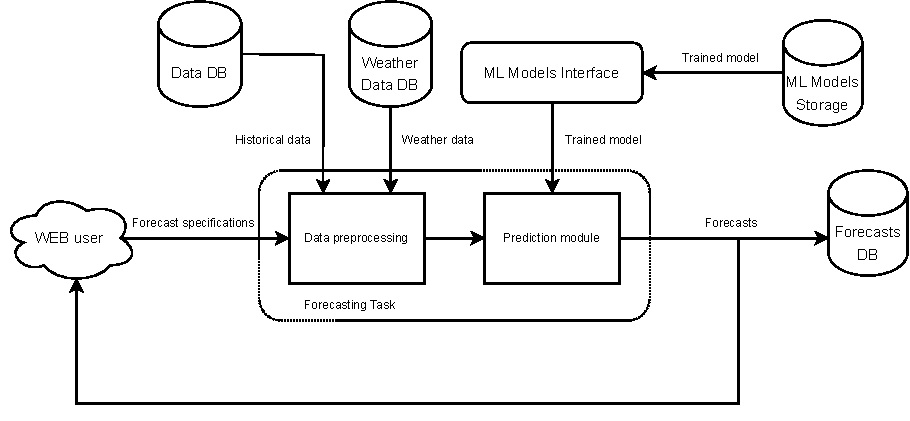
\includegraphics[width=0.6\textwidth]{images/architecture_forecasting_flow}
\caption{Diagram representing the forecasting flow.}
\label{fig:forecastflow}
\end{figure}

The sequence diagram representing the complete forecasting procedure for a specific use case is presented in figure~\ref{fig:forecastingsequence}.

\begin{figure}[H]
\centering
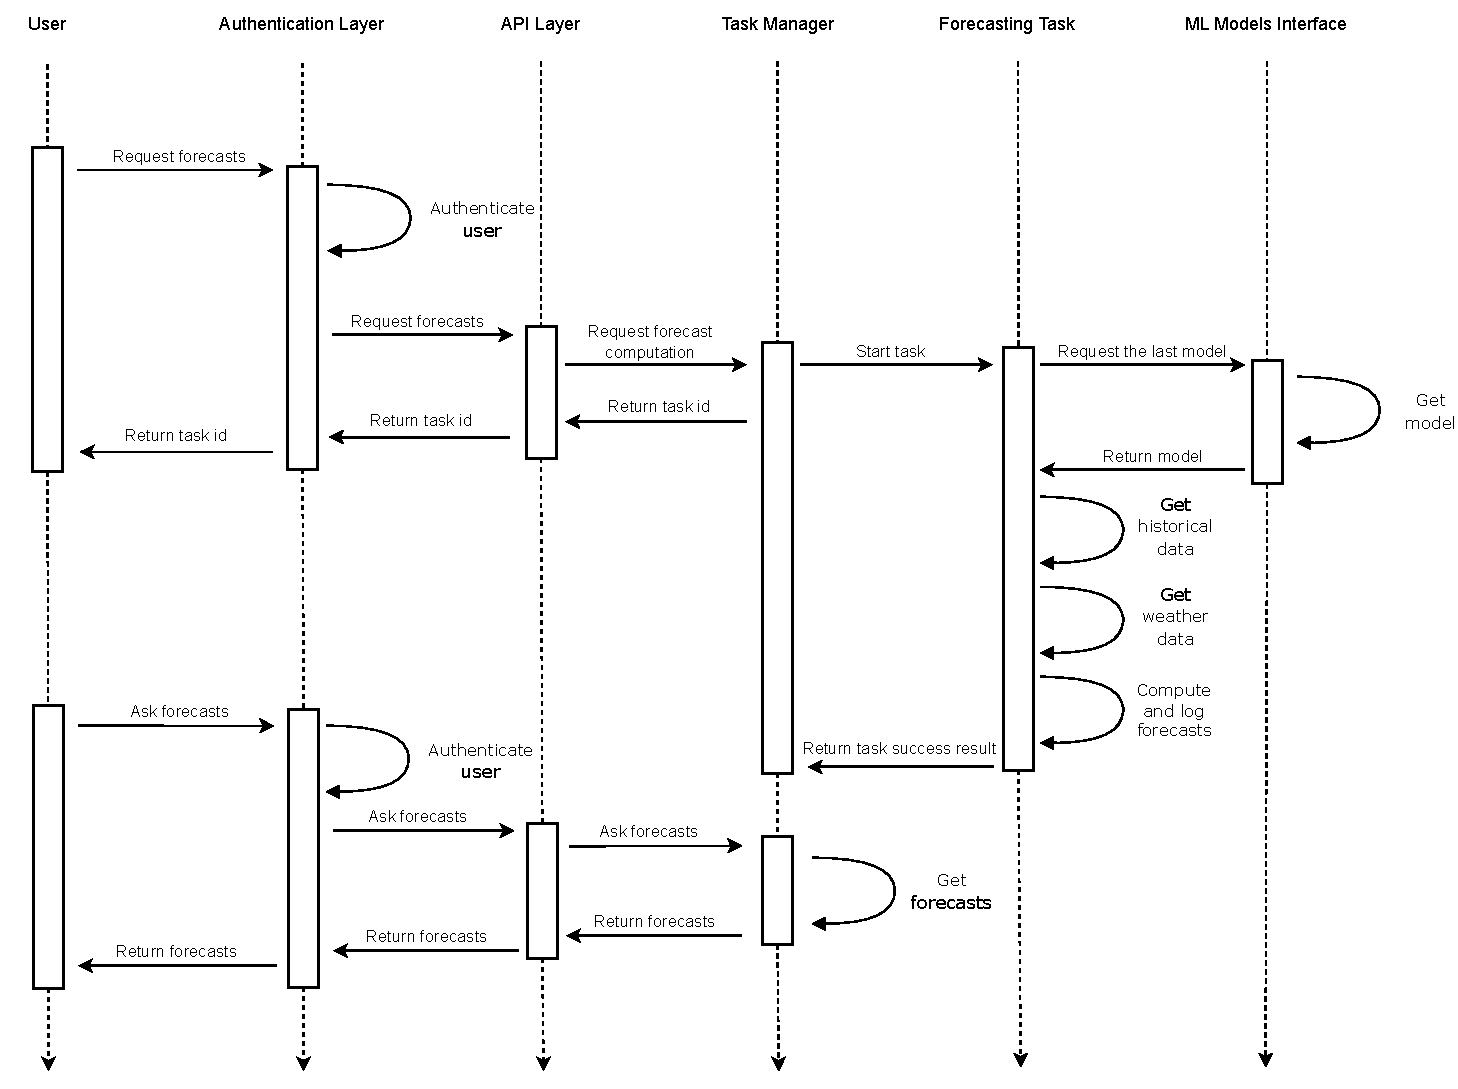
\includegraphics[width=0.8\textwidth]{images/architecture_forecasting_sequence}
\caption{Sequence diagram representing the forecasting procedure.}
\label{fig:forecastingsequence}
\end{figure}


\vspace{0.1 cm}
\subsection{Performance evaluation}
\label{sec:scheduler}
\vspace{0.1 cm}

The diagram representing the components' interactions for achieving the performance evaluation use case is presented in figure~\ref{fig:schedulerinteractions}.

The task scheduler periodically creates and triggers a performance evaluation task.
As shown by the diagram in figure~\ref{fig:schedulerflow}, the logic inside the performance evaluation task can be formulated in 2 steps: preprocess the data and evaluate the performance.
The data preprocessing block collects the data for the specific use case for which the model will be trained, aggregates it correctly, cleans it, and enriches it with weather data.
The performance evaluation module takes the preprocessed data and evaluates the performance of the last available models.
The performance evaluation procedure with the obtained results is described in chapter~\ref{cha:evaluation}.
When performance drops significantly, it triggers the models re-training by creating a model training task for having up-to-date models with respect to the user data so that they might perform better on future forecasts.
The model training task is described more in detail in subsection~\ref{sec:training}.

\begin{figure}[H]
\centering
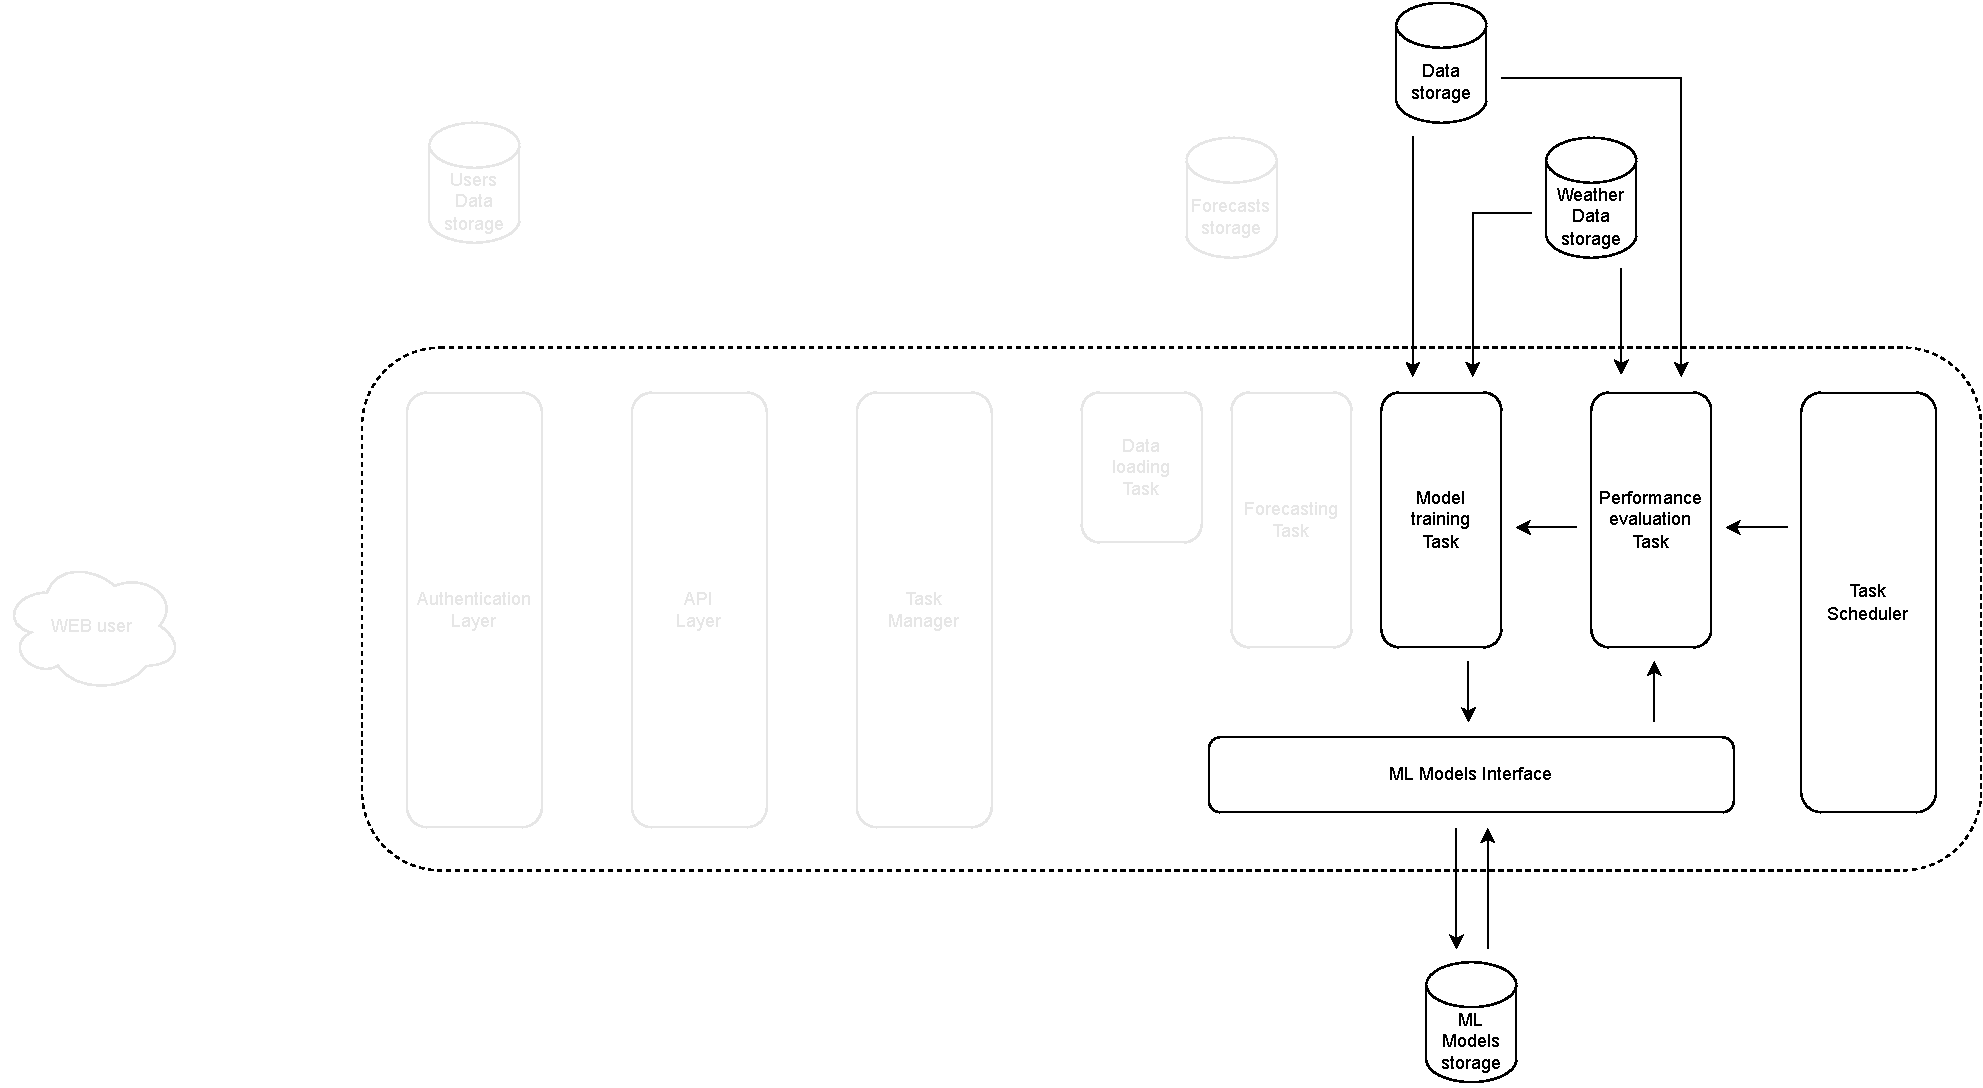
\includegraphics[width=1\textwidth]{images/architecture_scheduler_interactions}
\caption{The interactions among the components for achieving the performance evaluation use case.}
\label{fig:schedulerinteractions}
\end{figure}

\begin{figure}[H]
\centering
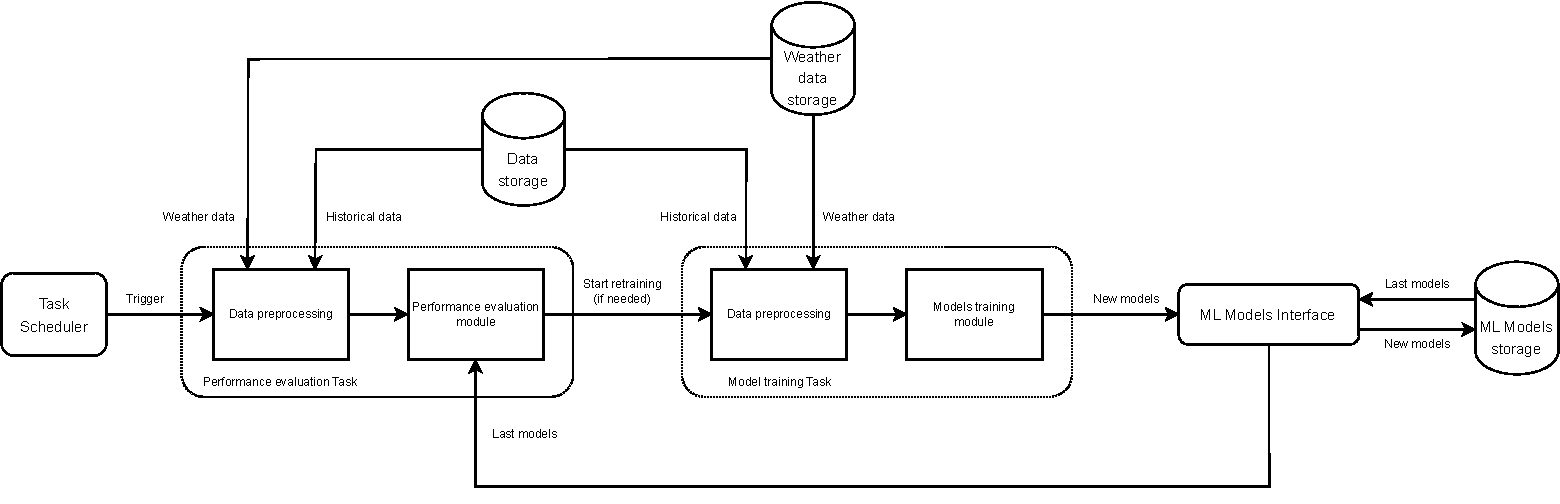
\includegraphics[width=1\textwidth]{images/architecture_scheduler_flow}
\caption{Diagram representing the performance evaluation flow.}
\label{fig:schedulerflow}
\end{figure}

The sequence diagram representing the complete performance evaluation procedure is presented in figure~\ref{fig:schedulersequence}.

\begin{figure}[H]
\centering
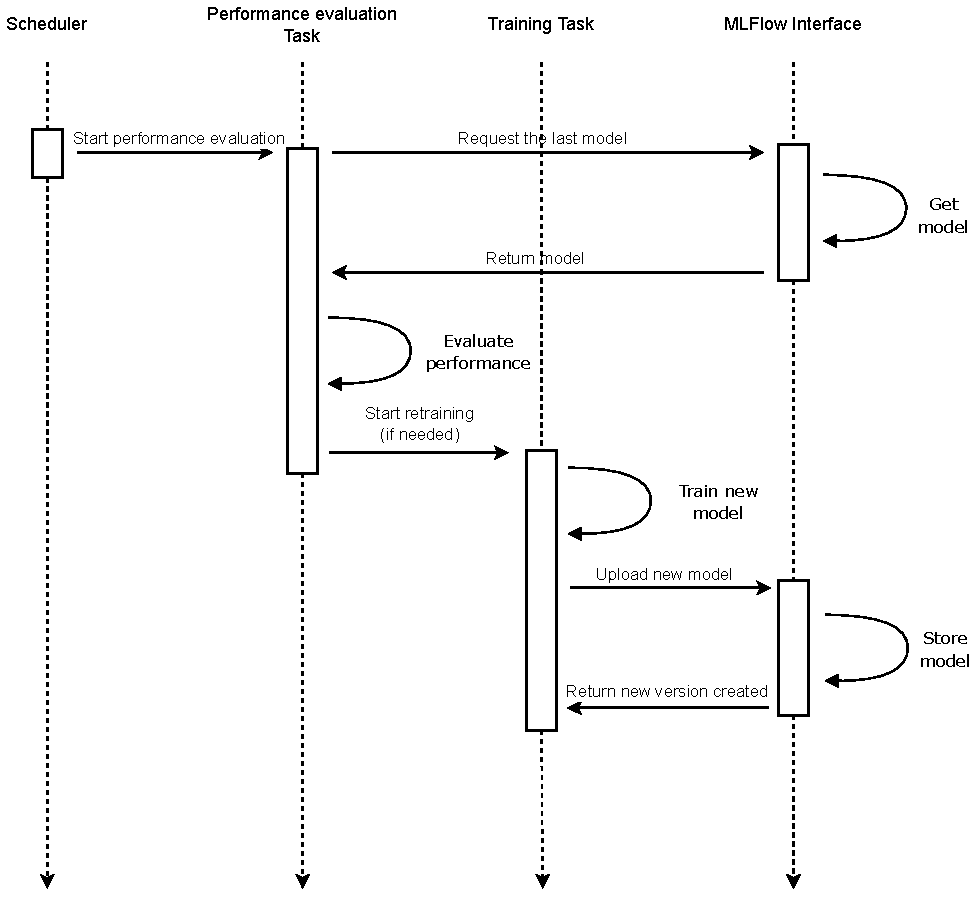
\includegraphics[width=0.6\textwidth]{images/architecture_scheduler_sequence}
\caption{Sequence diagram representing the performance evaluation procedure.}
\label{fig:schedulersequence}
\end{figure}


\section{System's common components}
\label{sec:components}
\vspace{0.2 cm}

In this section, the system's common components across the various specific use cases are described in detail.

The authentication layer manages the user authentication process.
In particular, for accessing the system the user needs to be authenticated.
When users interact with the system via dedicated APIs, to be authorized they must provide one valid token and have an account with an active subscription.
It is also possible to have more users associated with the same account.

The API layer manages the user interactions with the system.
Many endpoints are available for managing the users' possible operations, such as data loading, model training, and forecasting requests.
Data loading management endpoints consist of requesting the loading of new data and checking the status of the data loading operations.
Model training management endpoints consist of requesting the training of new models and checking the status of the model training operations.
Forecasting requests management endpoints consist of requesting the forecasts of future data and checking the status of the forecasting requests operations.

The task manager coordinates the execution of the different tasks requested by the users.
Where the possible tasks, as described in the previous section, are the following:
\begin{itemize}
  \item Data loading task, which parses and stores the users' loaded data on the basis of the type of data;
  \item Model training task, which trains new models based on available data. The specialization of this task for the specific use cases is described in the dedicated sections;
  \item Forecasting task, which forecasts future data using a specified model. The specialization of this task for the specific use cases is described in the dedicated sections.
\end{itemize}

For the data loading task, the main blocks are:
\begin{itemize}
  \item Data parser, which transforms the input user data in a system-compatible format, the expected information in data depends on the specific use case for which data is loaded;
  \item Data storage, which stores the parsed data inside the data storage with a create or update logic specifying the type of data.
\end{itemize}

The base blocks across the various specific use cases that are then described more in detail in the following sections are the following:
\begin{itemize}
  \item Data preprocessing, which retrieves the needed data from the data storage, aggregates it correctly, cleans it by filling the gaps by using a linear interpolation, and enriches it using the weather information retrieved from the weather data storage. For future data forecasts in addition to past weather data also weather forecasts are collected;
  \item Models training module, which takes the preprocessed data and trains the specified model with the provided specifications;
  \item Prediction module, which takes the preprocessed data, requests the specified model, and computes the forecasts.
\end{itemize}

The ML model interface handles the interactions with the ML models storage where the trained ML models are stored.
In particular, this component provides the functionalities to store and retrieve models in the ML models storage,
This component allows the system to support lots of models for each account and new ones can be added over time.
A versioning mechanism is also handled in the model storage.
This component allows the system to provide users with the latest available models and choose the best-performing ones.

The task scheduler manages the periodic scheduled tasks.
In particular, as described in the previous section, it is present just the performance evaluation task, which evaluates the performance of the available models and if needed triggers the models re-training.
The main block of this task is the performance evaluation module, which takes the preprocessed data and evaluates the performance of the last available models using specific use case error metrics such as MAPE and MAE.


\section{Electricity demand forecasting module}
\label{sec:demandmodel}
\vspace{0.2 cm}

In this section, the electricity demand forecasting module is described.
The module handles the specialization of data models, training, and forecasts for the electricity demand forecasting use case.

The UML (Unified Modeling Language) data class for electricity demand forecasting is represented in figure~\ref{fig:umldemand}.
The considered attributes are the following: the date and time of the detection, the active incoming to the customers in the past hour, and the number of customers.
The basic data is enhanced with the following weather information, the reported value is the average of the value in the last hour: air temperature, apparent temperature, and relative humidity.
The mean active incoming per customer is calculated as the division of the total active incoming by the number of customers.

\begin{figure}[H]
\centering
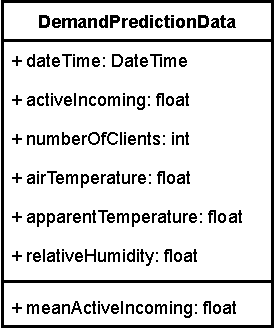
\includegraphics[width=0.20\textwidth]{images/demand_prediction_uml}
\caption{The UML data class for electricity demand forecasting.}
\label{fig:umldemand}
\end{figure}

The schematic representation of the model training procedure for electricity demand forecasting is presented in figure~\ref{fig:modeltrainingdemand}.
It consists of 2 modules: the data preprocessing module and the models training module.
The data preprocessing module takes historical aggregated consumption data and historical weather data as input and prepares the data for the model training.
The models training module based on the prepared data trains the set of available models for electricity demand forecasting: SARIMA, support vector regressor, hist gradient boosting regressor, extreme gradient boosting regressor, prophet, LSTM, GRU, CNN, TFT, and the combination of different techniques which is also tested.
Some baseline approaches which consider repeating past days and weeks, and an AutoML approach are also considered as comparisons.

\begin{figure}[H]
\centering
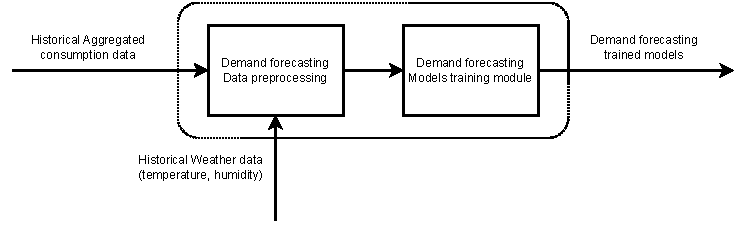
\includegraphics[width=0.7\textwidth]{images/system_model_training_demand}
\caption{The schematic representation of the model training procedure for electricity demand forecasting.}
\label{fig:modeltrainingdemand}
\end{figure}

The schematic representation of the forecasting procedure for electricity demand forecasting is presented in figure~\ref{fig:modelforecastingdemand}.
It consists of 2 modules: the data preprocessing module and the prediction module.
The data preprocessing module takes forecast specifications, historical aggregated consumption data, historical weather data, and weather forecasts as input and prepares the data for the forecasting.
The prediction module based on the prepared data computes the aggregated demand forecasts for the trained available models.

\begin{figure}[H]
\centering
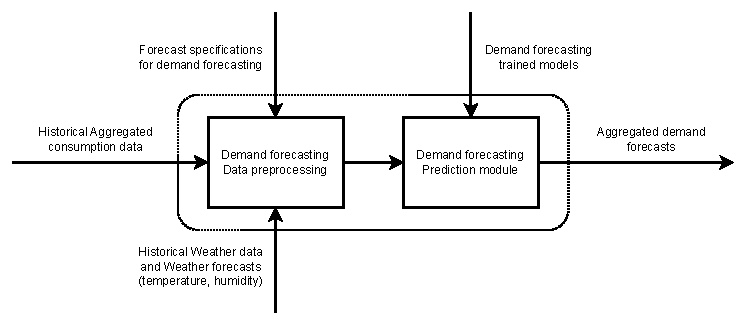
\includegraphics[width=0.7\textwidth]{images/system_model_forecasting_demand}
\caption{The schematic representation of the forecasting procedure for electricity demand forecasting.}
\label{fig:modelforecastingdemand}
\end{figure}


\section{Consumption baseline forecasting module}
\label{sec:baselinemodel}
\vspace{0.2 cm}

In this section, the consumption baseline forecasting module is described.
The module handles the specialization of data models, training, and forecasts for the consumption baseline forecasting use case.

The UML data class for consumption baseline forecasting is represented in figure~\ref{fig:umlbaseline}.
The considered attributes are the following: the date and time of the detection, the CUPS code (Universal Supply Point Code) which identifies the customer, and the active incoming to the customer in the past hour.
In the case of other customer information, this might be used to try to improve the performance of the models.
The basic data is enhanced with the following weather information, the reported value is the average of the value in the last hour: air temperature, apparent temperature, and relative humidity.

\begin{figure}[H]
\centering
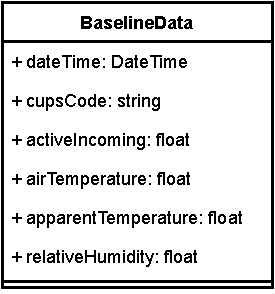
\includegraphics[width=0.20\textwidth]{images/baseline_uml}
\caption{The UML data class for consumption baseline forecasting.}
\label{fig:umlbaseline}
\end{figure}

The schematic representation of the model training procedure for consumption baseline forecasting is presented in figure~\ref{fig:modeltrainingbaseline}.
It consists of 2 modules: the data preprocessing module and the models training module.
The data preprocessing module takes historical single customer consumption data and historical weather data as input and prepares the data for the model training.
The models training module based on the prepared data trains the set of available models for consumption baseline forecasting: SARIMA, support vector regressor, hist gradient boosting regressor, extreme gradient boosting regressor, prophet, LSTM, GRU, CNN, and TFT.
Some baseline approaches which consider repeating past days and weeks, and an AutoML approach are also considered as comparisons.

\begin{figure}[H]
\centering
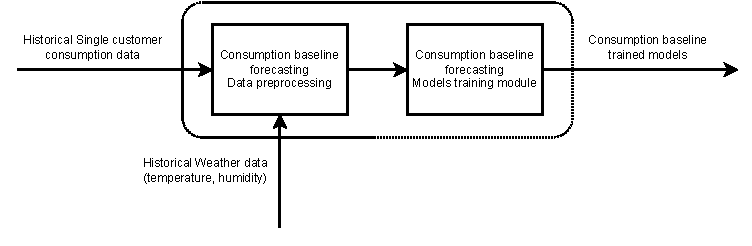
\includegraphics[width=0.7\textwidth]{images/system_model_training_baseline}
\caption{The schematic representation of the model training procedure for consumption baseline forecasting.}
\label{fig:modeltrainingbaseline}
\end{figure}

The schematic representation of the forecasting procedure for consumption baseline forecasting is presented in figure~\ref{fig:modelforecastingbaseline}.
It consists of 2 modules: the data preprocessing module and the prediction module.
The data preprocessing module takes forecast specifications, historical single customer consumption data, historical weather data, and weather forecasts as input and prepares the data for the forecasting.
The prediction module based on the prepared data computes the single customer consumption baseline forecasts for the trained available models.

\begin{figure}[H]
\centering
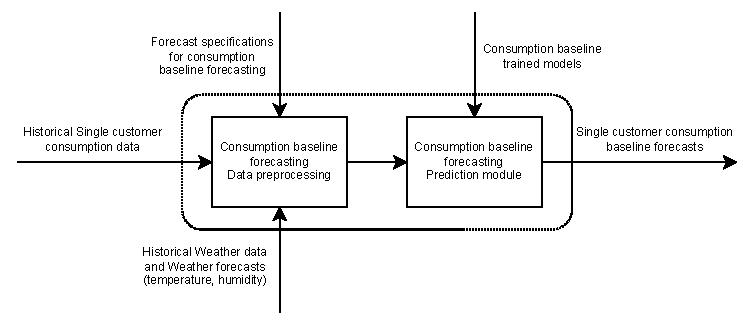
\includegraphics[width=0.7\textwidth]{images/system_model_forecasting_baseline}
\caption{The schematic representation of the forecasting procedure for consumption baseline forecasting.}
\label{fig:modelforecastingbaseline}
\end{figure}


\section{Electricity production forecasting module}
\label{sec:productionmodel}
\vspace{0.2 cm}

In this section, the electricity production forecasting module is described.
The module handles the specialization of data models, training, and forecasts for the electricity production forecasting use case.

The UML data class for a single PV plant data for electricity production forecasting is represented in figure~\ref{fig:umlsingleplant}.
The considered attributes are the following: the date and time of the detection, the id of the asset (intended as the PV plant identifier), the nominal power of the PV plant (intended as its maximum theoretical production power per hour), and the produced energy in the past hour by the PV plant.
The basic data is enhanced with the following weather information, the reported value is the average of the value in the last hour: air temperature, apparent temperature, relative humidity, wind speed, wind direction, pressure altimeter, visibility, sky coverage, diffuse horizontal irradiance, direct normal irradiance, global horizontal irradiance, solar radiation, UV index, solar elevation angle, and solar azimuth angle.
The percentage of production is calculated by the division of the produced energy by the nominal power of the PV plant.

While the UML data class for the aggregated data over PV plants for electricity production forecasting is represented in figure~\ref{fig:umlproduction}.
The considered attributes are the following: the date and time of the detection, the number of PV plants, the total nominal power of the PV plants (intended as the sum of the maximum theoretical production power per hour of all PV plants), and the produced energy in the past hour by the PV plants.
The basic data is enhanced with the following weather information, the reported value is the average of the value in the last hour: air temperature, apparent temperature, relative humidity, wind speed, wind direction, pressure altimeter, visibility, sky coverage, diffuse horizontal irradiance, direct normal irradiance, global horizontal irradiance, solar radiation, UV index, solar elevation angle, and solar azimuth angle.
The mean produced energy for a single PV plant is calculated as the division of the total produced energy by the number of PV plants.
The mean percentage of production is calculated as the division of the total produced energy by the total nominal power of the PV plants.

\begin{figure}[H]
\begin{minipage}[b]{8.5cm}
\centering
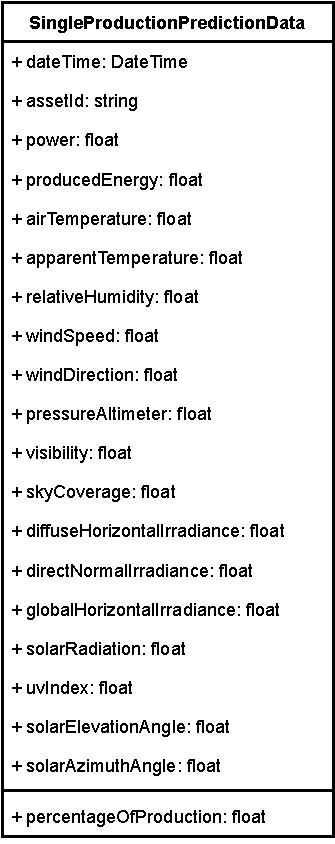
\includegraphics[width=0.45\textwidth]{images/single_plant_uml}
\subcaption{}
\label{fig:umlsingleplant}
\end{minipage}
\ \hspace{2mm} \
\begin{minipage}[b]{8.5cm}
\centering
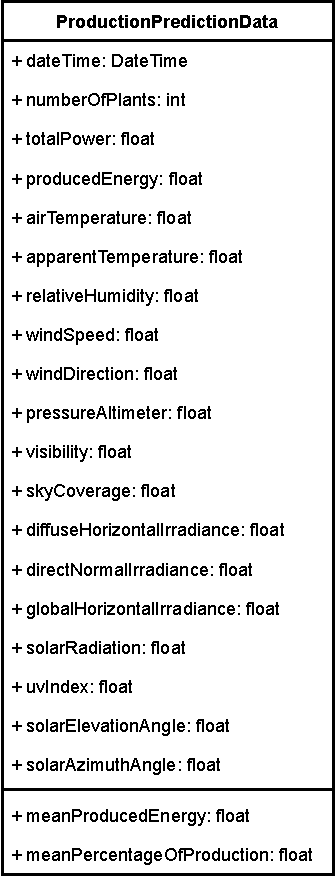
\includegraphics[width=0.45\textwidth]{images/production_prediction_uml}
\subcaption{}
\label{fig:umlproduction}
\end{minipage}
\caption{\subref{fig:umlsingleplant} The UML data class for a single PV plant data and \subref{fig:umlproduction} the UML data class for the aggregated data over PV plants for electricity production forecasting.}
\end{figure}

The schematic representation of the model training procedure for electricity production forecasting is presented in figure~\ref{fig:modeltrainingproduction}.
It consists of 2 modules: the data preprocessing module and the models training module.
The data preprocessing module takes historical PV plants production data and historical weather data as input and prepares the data for the model training.
The models training module based on the prepared data trains the set of available models for electricity production forecasting: ARIMA, support vector regressor, hist gradient boosting regressor, extreme gradient boosting regressor, prophet, LSTM, GRU, CNN, TFT, and the combination of different techniques which is also tested.
A baseline approach which considers repeating past days and an AutoML approach are also considered as comparisons.

\begin{figure}[H]
\centering
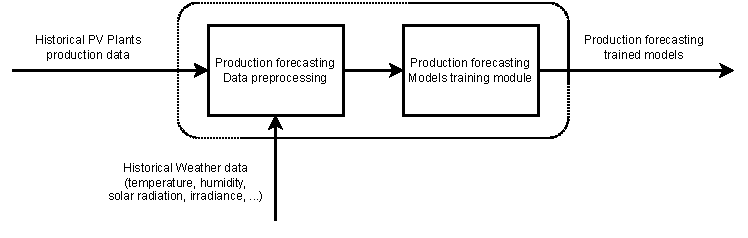
\includegraphics[width=0.7\textwidth]{images/system_model_training_production}
\caption{The schematic representation of the model training procedure for electricity production forecasting.}
\label{fig:modeltrainingproduction}
\end{figure}

The schematic representation of the model training procedure for electricity production forecasting is presented in figure~\ref{fig:modelforecastingproduction}.
It consists of 2 modules: the data preprocessing module and the prediction module.
The data preprocessing module takes forecast specifications, historical PV plants production data, historical weather data, and weather forecasts as input and prepares the data for the forecasting.
The prediction module based on the prepared data computes the aggregated PV plants production forecasts for the trained available models.

\begin{figure}[H]
\centering
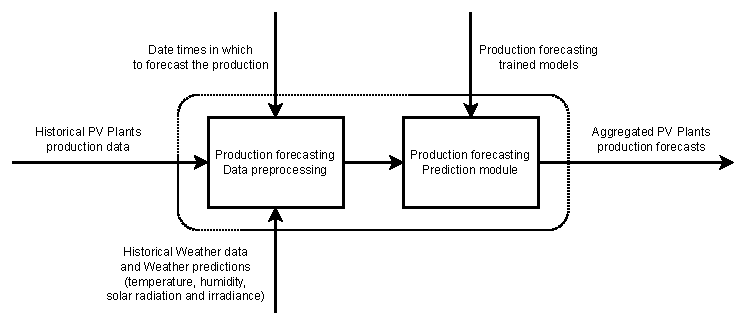
\includegraphics[width=0.7\textwidth]{images/system_model_forecasting_production}
\caption{The schematic representation of the model training procedure for electricity production forecasting.}
\label{fig:modelforecastingproduction}
\end{figure}
